\documentclass[12pt, a4paper]{article}
\usepackage{amsmath}
\usepackage[english]{babel}
\usepackage{graphicx}
\usepackage{caption}
\usepackage{xcolor}
\usepackage{float}
\usepackage{amssymb}
\usepackage{subfig}

\newcommand{\diff}[2]{\frac{\partial{#1}}{\partial{#2}}}
\newcommand{\todo}{\textcolor{red}{\textbf{TODO:}}}
\newcommand{\R}{\mathbb{R}}
\newcommand{\norm}[1]{\parallel{#1}\parallel}
\newcommand{\img}[4]{\includegraphics[scale={#4}]{./plots/#1/#2/#3}}

\newcommand{\tablePlot}[3][.3]{\begin{figure}[H]
\subfloat[obstacle: \textbf{far}, control points always active]{\img{far}{always}{#2}{#1}}\hfill
\subfloat[obstacle: \textbf{near}, control points always active]{\img{near}{always}{#2}{#1}}\hfill
\subfloat[obstacle: \textbf{on path}, control points always active]{\img{on}{always}{#2}{#1}}\\
\subfloat[obstacle: \textbf{far}, control points \emph{not} always active]{\img{far}{notAlways}{#2}{#1}}\hfill
\subfloat[obstacle: \textbf{near}, control points \emph{not} always active]{\img{near}{notAlways}{#2}{#1}}\hfill
\subfloat[obstacle: \textbf{on path}, control points \emph{not} always active]{\img{on}{notAlways}{#2}{#1}}
\caption{#3}
\end{figure}}

\begin{document}
	
	\title{Task Priority Matrix method with collision avoidance}
	\author{Stefano De Filippis \& Marco Menchetti}
	\date{October 2019}
	\maketitle
	
	\newpage
	\tableofcontents
	
\begin{abstract}
	\textbf{
	In this project we will face the problem of task priority resolution using a fast computation of the priority matrix (here \textit{Flacco Matrix}) and the resulting joint velocities.}

\textbf{
	Collision avoidance for several control points has been taken as a high priority task in this case as well as trajectory tracking.}
\end{abstract}
%\begin{keywords}
%	Priority; Task Priority; Collision Avoidance	
%\end{keywords}
\section*{Introduction}
Due to their high dexterity and the absence of non-holonomic constraints, manipulators has been used to perform a wide range of operation, and sometimes even more of them at the same time.

A handy yet practical example is the one considered below: a manipulator moving in a cluttered environment, trying to complete a trajectory tracking task and, at the same time, avoid collision with obstacles nearby.

\section{Tasks definition}
The tasks we used are four and they occupy 6 out of 7 manipulator's DOF:
\begin{itemize}
	\item one Cartesian positioning task occupying 3 DOF.
	\item one link orientation task for the third link axis, which occupies 1 DOF.
	\item two control points' collision avoidance tasks that will occupy overall 2 DOF.
\end{itemize}
\subsection[Task 1]{Cartesian positioning}
The Cartesian positional task is defined by the direct kinematics of the robot as:
\[r_d = f(q)
\] which is used to compute the task analytical Jacobian and the task error, $e = r_d - r$. Hence it's straight-forward the expression of this task's associated velocity: 
\begin{equation}
\label{EQN: task1}
 \dot{r_d} = \diff{f(q)}{q} \dot{q} = J\dot{q}
\end{equation}
so as 
\[\dot{q} = J^{\#}\dot{r_d}
\]

\subsubsection{Collision avoidance}
In the formulation of our problem, where $\dot{r}$ is given (i.e. precalculated), we are left with finding the right value for $\dot{q}$.

As already said, in our approach, we have also to include the collision avoidance for the end-effector. Instead of treating it as a different task, as we will do for the other control points, we could handle it in a "tricky" way so as to not saturate other DOFs: we will use instead of $\dot{r}$, the \textbf{sum} between $\dot{r}$ and another Cartesian velocity, $\dot{r_o}$, pushing the end-effector away from the obstacle. This Cartesian velocity will be directed as the distance from the center of the obstacle to the tip of the manipulator, and will have a magnitude weighted by a non-linear gain $v(P,O)$, where $P = f(q)$ is the end-effector position and $O$ is the obstacle position.
Hence:
\begin{equation}\label{repulsive_dir}
\dot{r_o} = v(P,O)\frac{f(q) - O}{\lVert f(q) - O \rVert}
\end{equation}
\begin{equation}\label{repulsive_mag}
v(P,O) = \frac{V_{max}}{1+e^{(\lVert f(q) -O \rVert(2/\rho)-1)\alpha}}
\end{equation}

In the end we will have \eqref{EQN: task1} in the form: 
\[
\dot{r_d} + \dot{r_o} = J\dot{q} \rightarrow \dot{q} = J^{\#}(\dot{r_d}+\dot{r_o})
\]
\subsection[Task 2]{Desired link orientation}
About Cartesian orientation, we want to keep the third link axis vertical, hence we need to attach a vector $p_l$ to this axis:
\[
p_l = p_5(q) - p_4(q) \rightarrow p_l(q)
\]
Where $p_5(q)$ and $p_4(q)$ are the 4$^{th}$ and 5$^{th}$ DH reference frames' origin.

We are interested in keeping the elevation, $\phi$, of this link vertical. Transforming $p_l(q)$'s coordinates from Cartesian to spherical, we can express this second task as:
\[
r_2 = \phi(q) = \text{arccos}(\frac{p_{l,z}(q)}{\norm{p_l(q)}})
\]
Using $d_l(q) = \frac{p_{l,z}(q)}{\norm{p_l(q)}}$, we can more practically compute its associated Jacobian as:
\begin{equation}
J_2 = \diff{\text{arccos}(d_l)}{d_l}\diff{d_l}{q}\dot{q}
\end{equation}
%And, computing each block independently we get that:
%\begin{align}
%\diff{\phi}{p} &= \frac{-1}{\sqrt{1-p^2}}\\
%\diff{p}{q} &= \frac{p_{l,z}(q)^{'}\norm{p_l(q)} - p_{l,z}(q)\norm{p_l(q)}^{'}}{\norm{p_l(q)}^2} \nonumber \\
%&= (\frac{\hat{z}^T\norm{p_l(q)}^2 - p_{l,z}(q)p_l(q)^T}{\norm{p_l(q)}^3})\begin{bmatrix}
%J_5 - J_4
%\end{bmatrix}
%\end{align}
%Where we know that $p_{l,z}(q)^{'}$ and $\norm{p_{l}(q)}^{'}$ are defined as below, using $\hat{z}^T = \begin{bmatrix}
%0&0&1
%\end{bmatrix}$.
%\begin{align*}
%p_{l,z}(q)^{'}&= \diff{p_{l,z}(q)}{q} = \hat{z}^T\begin{bmatrix}
%J_5 - J_4
%\end{bmatrix} \\
%\norm{p_l(q)}^{'}&=\diff{(\norm{p_l(q)})}{q}= \frac{p_{l,z}(q)p_l(q)^T}{\norm{p_l(q)}}\begin{bmatrix}
%J_5-J_4
%\end{bmatrix}
%\end{align*}


\subsection[Tasks 3 \& 4]{Control points' collision avoidance}
When dealing with the collision avoidance task linked to the two control points we were left with only 2 DOFs for both so we had to use one for each point. We couldn't use the same approach we used for the end-effector but at the same time something rather similar has to be done. 

To compress the three DOFs into one, we projected the collision avoidance task velocity, $\mathbf{\dot{r_{o}}_{,i}}$ computed as in \eqref{repulsive_dir} but using the control point position $P_c$ as $P$, onto the direction of the velocity itself. In this way we get a task velocity which is a scalar (1 DOF) equal to the magnitude of the original one (i.e. \eqref{repulsive_mag}).

Defining 
\begin{itemize}
	\item $\eta = \frac{P_c - O}{\norm{P_c-O}}$
	\item $P_c$ as the control point's position
	\item $O$ as the position of the obstacle
	\item $J_i$ as the analytical jacobian associated to the $i^{th}$ control point
\end{itemize}
we end up with:
\begin{equation*}
\eta^T\dot{r_{o}}_{,i} = v(P_c,O) =\eta^T J_i\dot{q} = J_{c,i}\dot{q}
\end{equation*}
Hence:
\begin{equation}
v(P_c,O) = J_{c,i}\dot{q} \rightarrow \dot{q} = J_{c,i}^{\#}v(P_c,O)
\end{equation}

\subsubsection{Points' positioning}

For this particular manipulator we chose 3 control points:
\begin{enumerate}
\item The first is on the tip of the end-effector.
\item The second is on the origin of the DH frame associated to the 4$^{th}$ joint (i.e. on the "elbow").
\item The third is on the second link axis at a given distance from the origin of the DH reference frame associated to the 2$^{nd}$ joint (i.e. half link axis' length off the shoulder). In that reference frame, its position is:
\[c_{pt,3} = \begin{bmatrix}
0\\0\\ \frac{d_1}{2}
\end{bmatrix} = \begin{bmatrix}
0\\0\\ 0.2
\end{bmatrix}
\]
\end{enumerate}
\section{Control architecture}
Due to the high complexity of the task we divided our control scheme into 3 main blocks:
\begin{enumerate}
	\item \textbf{Priority matrix:} to compute in a fast way the joint velocities executing the task ones, coming from the prioritized stack of tasks.
	\item \textbf{Priority resolution algorithm:} to organize the stack of tasks accordingly to each ones' \textit{generalized cost}.
	This concept will be further explained below.
	\item \textbf{Control algorithm:} to merge both the above methods and generate a desired joint velocity.
\end{enumerate}

\subsection{Priority matrix}
\subsubsection{Redundancy Resolution Problem}
The redundancy resolution problem consists in finding the robot command in order to execute a series of tasks, usually organized in a Stack of Task.
More generally, considering $k$ a generic task, the problem can be formalized through an equality relation \[A_kx=b_k\]
with the matrix $A_k \in \R^{mk \times n}$, and the vector $b \in \R^{mk}$. $n$ is the Degree of Freedom (DoF) of the system, and $mk$ is the task dimension ($mk \geq n$). The solution $x \in \Bbb R^n$ represents the robot motion for accomplishing the task.
Taking into account a SoT, instead, the transformation matrix and task vector can be simply defined by doing:
\[A=\begin{bmatrix}
A_1^T & A_2^T & \dots & A_l^T
\end{bmatrix}
\]
and
\[b=\begin{bmatrix}
b_1^T & b_2^T & \dots & b_l^T
\end{bmatrix}
\]

Where matrix \textbf{A} has dimension $\sum_{k=1}^l m_k \times n$, and vector \textbf{b} has dimension $\sum_{k=1}^l m_k \leq n$.
And the problem can be formalized through an equality relation: \[Ax = b\]

\subsubsection{The Siciliano And Slotine Solution}

If more than one task needs to be executed at the same time, though, we need to define a certain priority of execution between them. One way to handle the priority is  to consider it as a strict execution order between tasks. A second approach, though, consists in handling the priority as a weight for the cost function that the solver has to minimize.
The most used solution to solve the redundancy resolution problem is obtained by projecting a task in the null space of higher priority task, as proposed by Siciliano and Slotine (1991). Starting with $P_0 = I$ (the $n \times n$ Identity matrix) and $x_0 = 0$ (the $n \times 1$ zero vector), the contribution of each task, from the highest priority task $k = 1$ to the lowest priority task $k = l$, is computed as:
\[
x_k = x_{k-1} + (A_kP_{k-1})^{\#}(b_k - A_kx_{k-1})
\]where \[
P_k = P_{k-1}-(A_kP_{k-1})^{\#}A_kP_{k-1}
\]
is the projector in the null space of the all tasks from 1 to $k$.
With the development of this project, instead, we were able to investigate a different redundancy resolution methodology presented by Flacco. This approach is fast thanks to recent technologies and moreover presents interesting properties that allows us to have a little more insights and control about the stack of tasks due to the separation of the redundancy resolution from the assignment of the correct priority order. 
\subsubsection{The Task Priority Matrix}

Taking into account a SoT composed by l tasks, the non prioritized solution is obtained by inverting the augmented task:
\[
\overline{x} = A^\#b\]
If all the tasks are linearly independent, then they do not conflict with each other and they will be correctly executed by computing a solution which is equal to the one computed by the Siciliano algorithm. Otherwise conflicting tasks need to be accommodated.
An important aspect of the base solution, though, is that the contribution of each task and the task null space, can be easily extrapolated from $A^\#$, and this information can be useful when tasks need to be reordered or for other purposes. On the other hand, all this knowledge is lost in the Siciliano solution due to the projection of a task in the null space of a linearly depended higher priority task. 
So, in order to gain all these information while still imposing the correct task priority we need to find a matrix \textbf{F} that is able to enforce the task priority, such that the solution computed as: \[x = A^\#Fb\]
will be the same as the solution of the Siciliano algorithm.
\textbf{F} will be called the task priority matrix and from the equation is visible that this approach is effectively able to separate the redundancy resolution step from the imposition of the priority order, making it simpler to gain information of the task state and reorder the tasks at each iteration.
\paragraph{\textit{Rank 1 Case Study:}}
In order to understand how \textbf{F} can be chosen and have an insight about the knowledge that can be extrapolated from $A^\#$  we will report a simple example involving rank-1 tasks (mono dimensional tasks).
Suppose we have a SoT composed by two rank-1 linearly dependent tasks $a_1x = b_1$ and $a_2x = b_2$ . Namely, $a_2 = da_1$ , with $d \in \R$.
The solution obtained by the Siciliano algorithm is:\[
x=\begin{bmatrix}
a_1^\# & 0 
\end{bmatrix}
\begin{pmatrix}
b_1 \\ b_2
\end{pmatrix}
\]
which is equivalent to $x = a_1^\#b_1$ and therefore I can see only the contribution of the first task in the solution while the second task’s is lost.
On the other hand, if we compute the solution without priority we obtain.
\[
\overline{x} = 
\begin{bmatrix}
a_1 \\ a_2
\end{bmatrix}^\#
\begin{pmatrix}
b_1 \\ b_2
\end{pmatrix} = 
\begin{bmatrix}
\frac{1}{1+d^2}a_1^\# & \frac{d}{1+d^2}a_1^\#
\end{bmatrix}
\begin{pmatrix}
b_1 \\ b_2
\end{pmatrix}
\]
where now is evident the contribution of both tasks in the computation of the solution.
Now we need to define a matrix \textbf{F}  such that the 2 solutions given by (2) and (3) are the same and this can be done by choosing the matrix as:
\[
F = \begin{bmatrix}
1 & 0 \\ d & 0
\end{bmatrix}
\]
and the solution with priority can be obtained by computing:
\[
x = 
\begin{bmatrix}
a_1 \\ a_2
\end{bmatrix}^\#F
\begin{pmatrix}
b_1 \\ b_2
\end{pmatrix}
=\begin{bmatrix}
a_1^\# & 0 
\end{bmatrix}
\begin{pmatrix}
b_1 \\ b_2
\end{pmatrix}
\]
\paragraph{\textit{F General Structure:}}

By adding other tasks and by proceeding with the same comparing reasoning, can be shown that the F matrix display a particular structure:
\begin{itemize}
\item it is lower triangular;
\item it has ones on the diagonal, in correspondence of tasks linearly independent to higher priority tasks;
\item it has zeros on the diagonal, in correspondence of tasks linearly dependent to higher priority tasks;
\item it presents the coefficients of dependency in the left side of rows associated to tasks linearly dependent to higher priority tasks;
\end{itemize}
Moreover, the computation of this matrix can be easily done by computing the reduced row echelon form (rref) of $A^T$.
\paragraph{\textit{General Case:}}

When we consider tasks with dimension $>$ 1 then the task priority matrix still shows a similar structure to the one depicted above, but now single elements are substituted by square block matrices whose dimension is the same of the associated task. Then, taking a reasoning similar to the approach used in the rank-1 case, a tool similar to the rref for finding the tasks priority matrix \textbf{F} can be developed. The Gauss Jordan elimination is still used, as in rref, but considering pivot square matrices instead of pivot elements. Once again, the dimension of a pivot matrix is guided by the size of
the task.

\paragraph{\textit{The Algorithm:}} 

From now on we will refer to the general case and therefore we are going to develop a tool similar to the rref in order to obtain the Task Priority Matrix.
First is useful to use the QR decomposition of the augmented matrix \textbf{A} to compute its pseudoinverse.
\[
A^T = Q\begin{bmatrix}
R\\0
\end{bmatrix}
\]

From which the pseudoinverse is computed as $A^\# = QR^{-T}$. $R \in \R^{m\times m}$ is an upper triangular matrix that can be used to initialize the \textbf{F} matrix, while $Q \in \R^{n\times n}$.
As already mentioned in the previous section to obtain the priority task matrix we will perform the same steps of the Gauss Jordan elimination, but considering block matrices. Moreover, the all the operation are applied in place so at each step we will work on the modified matrix obtained at the previous step until we reach the final Task Priority Matrix.
So, at start we initialize the temporary \textbf{F} in the following way:
\[
\overline{F} = \bordermatrix{
~& m_1 & m_2 & & m_l\cr
m_1 & R_{11} & \star & \dots & \star \cr
m_2 & 0 & R_{22} & \dots & \star \cr
~ & 0 & 0 & \dots & \star \cr
m_l & 0 & 0 & \dots & R_{ll}
}
\]
where $m_{i-th}$ indicates the dimensions of the i-th tasks and the block pivot matrices are indicated explicitly, meanwhile the rest of the \textbf{R} matrix is not relevant.
From the properties of the QR decomposition, the diagonal blocks $\textbf{R}_{\textbf{kk}}$ is not singular if task \emph{k} is not singular and linearly independent to all tasks with higher priority.
Since the temporary \textbf{F} matrix is already upper triangular, Gauss Jordan elimination requires 2 steps for each task:
\begin{itemize}
\item First we need to set the pivot matrices to the Identity matrix by multiplying each block row with the pseudoinverse of its pivot matrix.
\item Then, all elements in the column block outside the diagonal should be set to zero. By considering the structure of the temporary matrix, and considering i<j, to nullify a block (i,j) by subtracting to the i-th row block the block (i,j) times the j-th row block. If after the first step the j-th pivot was an Identity matrix, then all elements in the block (i,j) are zeroed.
\end{itemize}
When all the steps are made for each task, then in order to get the Task Priority Matrix we will simply need to transpose the last temporary matrix obtained by the algorithm.
It is important to notice that in the first step just described we required the inverse of the pivot matrix, but since the k-th pivot matrix is only not singular if the k-th task is not singular and linearly independent from the higher order tasks we might not be able to do the inversion. Therefore, instead of the simple inversion we can use the pseudoinverse of the pivot matrix and in a damped version. Doing this we can obtain damped solutions that are better and smoother when we are reaching tasks' singularities.
\subsection{Priority resolution algorithm}
In this framework we will define:
\begin{enumerate}
\item[-] $O$ the position of the obstacle in the workspace.
\item[-] $D$ the distance from the obstacle for which we are more likely to end up in a dangerous situation.
\item[-] $d$ the distance from the obstacle which is quite dangerous but not yet critical.
\item[-] \texttt{stack} the array of Jacobians associated to each task.
\end{enumerate}
To keep a solution which is consistent with respect to our problem, we need an efficient resolution of the priority assignment and a meaningful cost for each task.
\subsubsection{Generalized cost}
In order to keep track of each task's priority, we need to organize our \texttt{stack}. Doing so requires to evaluate a cost function on the tasks for which the higher is the cost, the higher is the priority. Due to the fact that in this application all the tasks but the second, can be derived from the movement of a Cartesian point, we can use the distance of that particular point from the obstacle as our cost function.

As already said, unfortunately, the second task is not associated with any point, thus a decision has to be made: since we are not really interested in the execution of this task, we can simply say its cost is $d+1$, where we recall that \textit{d} is the \emph{dangerous distance} from the obstacle.

Doing so implies that this task will never overcome the others, which are associated with collision avoidance.


%Since in this application \textit{almost} each task is associated to the movement of a Cartesian point, we used the \textbf{distance} of that point from the obstacle.
%About \textit{task 2}, associated to a Cartesian orientation, we simply said it will have a constant cost computed as $d + 1$, so as to be always non-critical, this is due to the fact that we are not quite interested in the orientation task as we are in collision avoidance but we will also like that it is executed with a higher priority if we are in a normal operation point.

Note that many other choices for the cost could have been possible. Here a few that has been considered at the beginning:
\begin{list}{\textbf{Case:}}{}
\item Project the distance from the obstacle onto the instantaneous direction of motion for each control point, keep second task's cost constant.
\item Same as before but assign a control point to the midpoint of the third link to compute second task's cost.
\item Add and remove from the stack the task associated with control points.
\end{list}
\subsubsection{Priority assignment}

The assignment of the priority passes trough the reordering of the \texttt{stack} so as the task with priority $0$ will be the first element.
In this case we want to reorder the tasks differently based on the position of their associated point in the space.

We divided the \texttt{stack} into 2 sub-vectors whose dimensions, if summed, are \textbf{always} equal to the dimension of \texttt{stack} (i.e. the number of DOFs of the robot) and will be called \texttt{stack$_c$}, for the \emph{critic} part and \texttt{stack$_d$}, for both the \emph{dangerous} and \emph{normal} parts.

\begin{enumerate}
\item The points outside the \emph{dangerous} region won't be reordered.
\item the elements of \texttt{stack$_d$} in the \emph{dangerous} region will be reordered accordingly to their distance from $O$, if it's smaller than $D$ they will go into \texttt{stack$_c$}.
\item the elements of \texttt{stack$_c$} will be reordered accordingly to their distance from $O$.
\end{enumerate}
This will allows us to prioritize not only using the \emph{cost} but also the position of a task in the \texttt{stack}.

For example if we perform reordering using only the distance and all the control point are outside the \emph{dangerous} region except for one (e.g. $p_{c2}$), this will take over the priority of the Cartesian positioning task even if we would like to still execute the desired trajectory. While if we perform the \emph{critic-dangerous} distinction, and initialize the Cartesian positioning task to be always in \texttt{stack$_c$}, $p_{c2}$ will rise in the \texttt{stack}, up to the second position without overtaking the highest priority task.
\subsection{Control algorithm}
The control algorithm uses the block-scheme below.
\begin{figure}[H]
\centering
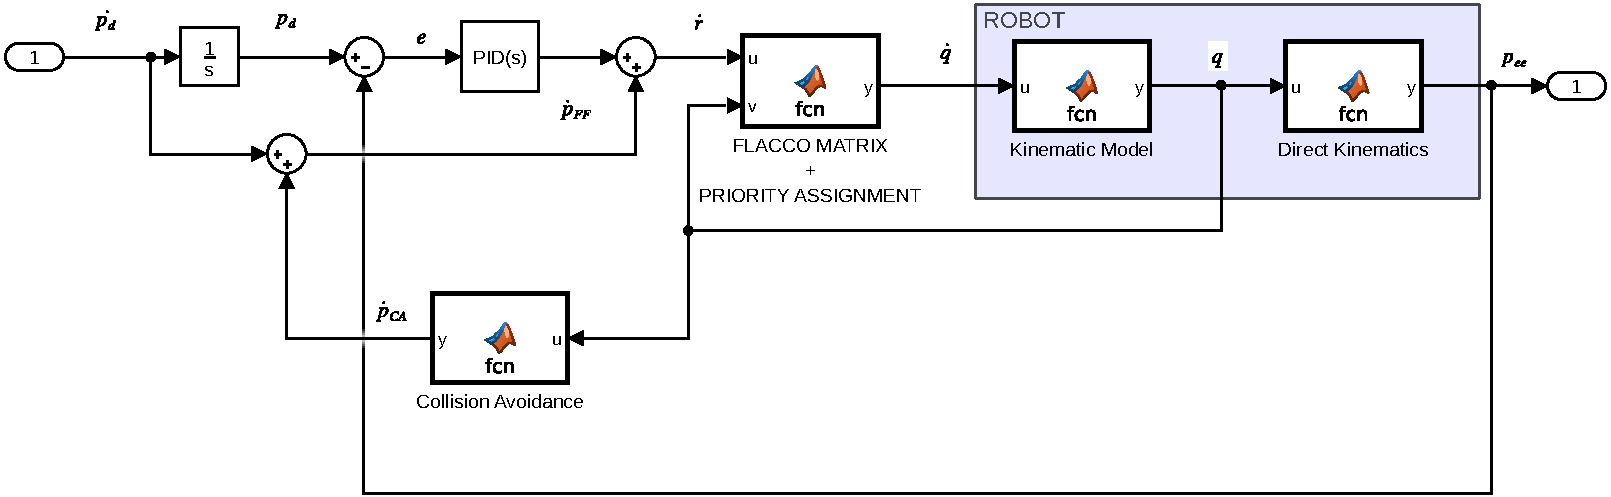
\includegraphics[width = 1.2\linewidth]{./plots/ControlSchemeModel.pdf}
\caption{Block scheme of the control architecture.}
\end{figure}
Which is a feedback plus feed-forward control architecture, where the feed-forward term is designed to achieve collision avoidance for the end-effector.

Note that all the information about the other control points and tasks are included into the \emph{Flacco Matrix} and into the task velocities' vector.
Those quantities have not been included since they are "known" at the control architecture's level and require no external reference.

\section{Results}
We organized the simulations accordingly with the distance of the end-effector from the obstacle and with its obstruction on the path. We simulated 3 different situations with 2 different control algorithms for a total of 6 different simulations.

In particular we used for the control algorithms:
\begin{enumerate}
\item The task associated with the control points are always present in the \texttt{stack}.
\item The task associated with the control points are kept away from the \texttt{stack} but their cost is evaluated at each iteration. Whenever they reach a certain threshold (here the control point get into the \emph{dangerous} region), they're added into the stack.
\end{enumerate}

While the simulations were divided into:
\begin{enumerate}
\item \textbf{Far:} The obstacle is located away and it does not interfere with the standard execution of the tasks.
\item \textbf{Near:} The obstacle is located near the path so as the end effector might get into the \emph{dangerous} region. However the most critical aspect comes from the fact that the last control point is inside the \emph{dangerous} region from the beginning.	
\item \textbf{On path:} The obstacle is located directly on the path, thus the there is no feasible motion for the end effector that realizes exactly the task. 
\end{enumerate}

\tablePlot[.33]{joint_angles}{Joint angles for the above cases:}
\subsection{Far obstacle.}
Although this might seem an useless case, it helps us to enlighten some fundamental differences between the two algorithm and unique characteristics of the prioritized solution. 

As figure 3 clearly shows, the standard execution of the task 1 \& 2 is way smoother when we include the task avoidance if strictly needed, and although the profile are the almost same the second solution provides joint velocities which have way lower magnitude. Take as an example joint 5 in figure 3d \& 3a.

Another interesting aspect is enlightened by figure 5 \& 6, where we can see that for both control algorithm, if possible, the error on the execution of all task is kept at the level of the least important task. This and the flexibility it offers are the reason why prioritizing tasks during the execution of motion is so important. 

\tablePlot[.33]{joint_velocities}{Joint velocities for the above cases:}
\subsection{Obstacle close to path.}
As already said, this particular choice of the obstacle position was meant to create a conflict in the control algorithm, on one side the end effector feels relatively safe with respect to the obstacle since its distance from it is quit large at the beginning, on the other hand the second control point stands right in the \emph{dangerous} region, hence the repulsive velocity it's subject to is quite strong even if it can't receive a higher priority, not being in the \emph{critical} region.

During the execution of motion however, in the final instants, also the ee gets inside that region, and it can be seen here the effect of the reordering algorithm:
\begin{itemize}
\item always keeping the control points in the \texttt{stack} biases the whole body to move away from the obstacle and we don't see any switching in the execution of this motion.
\item keeping the control points away while they're not needed, let them approach the obstacle and, as a matter of fact, we are required to switch the tasks since at least one of the control points get in the \emph{critical} region.
\end{itemize}

An interesting fact comes from the values the joint velocities assume for the first algorithm shows, for joints 5 \& 6, a mean which is almost zero, resulting in several inversion of motion through the whole simulation.

\tablePlot[.33]{control_points_distances}{Control points' distances for the above cases:}
\subsection{Obstacle on path.}

In this case the obstacle is placed directly on the path, and we can see that the error associated with the Cartesian positioning task is order of magnitude higher than all the previous case. A good test and proof for our control scheme is the fact that however big was this error we completed recovered it, and as soon as it has been possible we converged back to the path.

An interesting fact is that in this case, our problem might seem more difficult to solve while is indeed easier to handle. We can see that the control points almost never interact with the obstacle, hence the main discontinuities come from the tasks 1 and 2. The only time the control points start being problematic, is with the first algorithm when the second point gets too near to the obstacle and this result in a spike in joint velocities which gets smoothed quite fast.

\tablePlot[.33]{ee_task_error}{ee task error for the above cases:}
\section{Conclusion}

Those simulations provide quite interesting results which not always are overall decisive. A little note has to be made, using the first control algorithm, whenever a control point is outside the \emph{dangerous} region we are giving \emph{zero} velocity as a reference, thus the generally worst result. The whole body acts as if it is stiffer than it actually is, trying to keep fix the control points.

From an operative point of view it is clear why the prioritization of task is mandatory and how powerful it is the resulting flexibility in the control strategy. On the other hand some doubts arise on how effective it is to exploit the redundancies of a robot from the very beginning of a control action. 
For sure we can say that prioritization of tasks and null-space exploitation are two incredibly powerful tools which have to be handled carefully.
\tablePlot{elbow_task_error}{Elbow task error for the above cases:}

%\bibliography{sample}
%\bibliographystyle{ieeetr}

\end{document}
